\subsection{Results}
\label{sec:results}

\begin{figure}[htp]
\centering
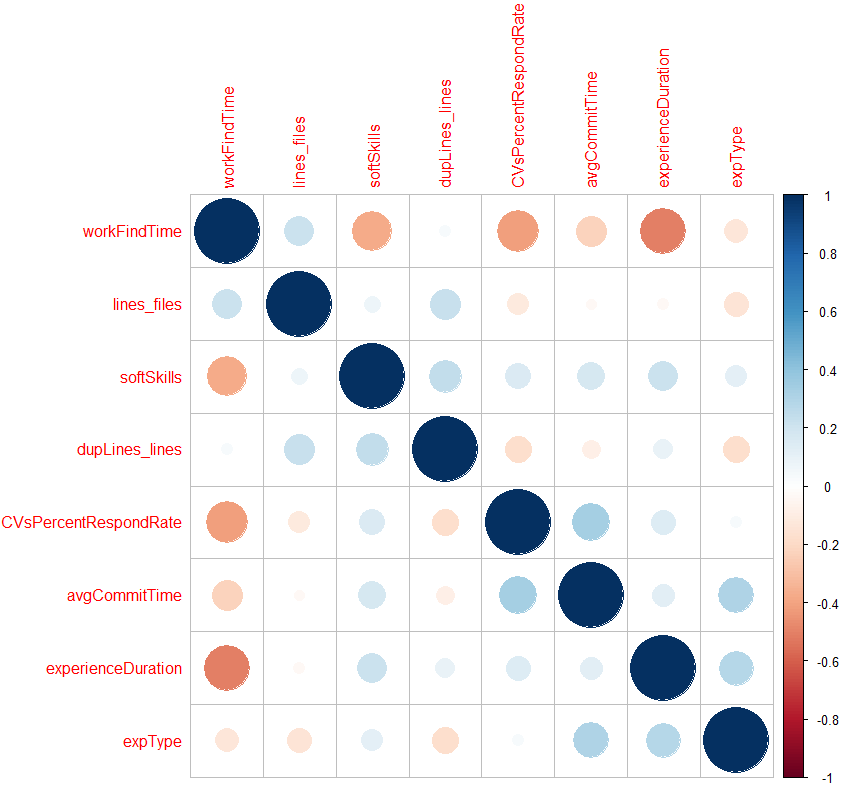
\includegraphics[width=\linewidth]{r_plot_corrrelation.png}
\caption{Correlation Matrix}
\label{fig:correlation-matrix}
\end{figure}

Uczenie modelu rozpoczeliśmy od zdefiniowania odpowiedniego task'a, w którym określiliśmy dane na podstawie których będzie budowany model oraz kolumnę targett, która określa czy dany użytkowik jest wart uwagi ze strony rekruterów. Do weryfikacji poprawności modelu wykorzystaliśmy repeated k-fold cross validation. Parametry walidacji przezentują sie następująco 4 foldy i 10 repeatów. 

Zdecydowaliśmy się na porówanie wyników dla trzech różnych modeli. Wyniki badań zaprezentowane są w tabeli poniżej (to w resultsach chyba).
\begin{center}
\begin{tabular}{ | m{5em} | m{5em}| m{5em} | m{5em}| m{5em} | m{5em}| } 
\hline
 Alghoritm & MMCE & MCC & F1 & ACC & Kappa\\ 
 \hline
 Random Forest & 0.329 & 0.245 & 0.410 & 0.671 & 0.219 \\ 
\hline
 SVM & 0.315 & 0.356 & 0.422 & 0.685 & 0.311 \\ 
\hline
 KNN & 0.388 & 0.224 & 0.431 & 0.611 & 0.184\\ 
\hline
\end{tabular}
\end{center}